\section{Development Model}
\label{sec:development}

To satisfy the mission of the Project, the SunPy community adopted an open development model, which is widely used within the scientific \python community.
The \sunpypkg package is hosted on \github and uses \code{git}\footnote{\url{https://git-scm.com/}} as its distributed version control software.
The entire code base is publicly available and anyone can suggest changes through pull requests.
Since the code base is licensed under a permissive 2-clause BSD license\footnote{\url{https://opensource.org/licenses/BSD-2-Clause}}, anyone can redistribute, improve, repackage or use it in a closed environment as long as they credit the SunPy developers and redistribute the license.
In order to maintain high-quality code, every contribution is reviewed and must satisfy the following requirements:
\begin{enumerate}
    \item Code and documentation must follow widely used style guides (e.g., PEP 8\footnote{\url{https://www.python.org/dev/peps/pep-0008/}}).
    \item All new features must be accompanied with documentation, including code comments, formal documentation such as \python docstrings and a guide, if appropriate, as well as gallery examples.
    \item Contributed code must provide unit tests\footnote{A unit test checks for the correct operation of a small component (or "unit") of the code base.} which cover the majority of the new functionality.
    \item All code must be within scope, and must be approved by at least two members of the developer community before it is merged into the code base\footnote{This requirement is relaxed for bug fixes or small documentation changes.}.
\end{enumerate}
These requirements are imposed on every pull request regardless of contributor.

As of version 1.0, \sunpypkg consists of 48,427 lines of code\footnote{This number includes documentation and comments.
There are 30,906 lines of code if documentation and comments are not counted.} contributed by 123 unique contributors with over 11,659 commits\footnote{A commit is a set of one or more modifications to the code base, with an associated description, and typically created by a single contributor.}.
The leftmost panel of \autoref{fig:metafig} shows the steady growth of the code base since 2011 with, on average, approximately 16 lines added per day.
A large reduction in the code base occurred after the release of 0.9, primarily due to the deletion of unused code and the removal of Python 2 support.

The middle panel of \autoref{fig:metafig} shows the steady rise in the number of unique contributors with, on average, more than one new contributor added each month.
The total number of contributors is large for a package of this size in the heliophysics community \citep{pyhc2018}.

The rightmost panel of \autoref{fig:metafig} shows the distribution of the total number of commits per contributor as of June 2019.
The distribution is relatively steep with a log-log slope of $-0.34$, which indicates that relatively few contributors generate the majority of commits.
The top 10 contributors are responsible for ${\sim}80\%$ of all commits.
This compares poorly to other projects such as \astropy \citep{astropy2018}.
Unlike \astropy, the \sunpyproj was not formed to bring together and coordinate many existing developers and their \python packages.
The development of the \sunpypkg package began by a core group of scientists with no prior existing code base.
It should be noted that the number of commits is only approximately related to contribution size since a single commit could include a substantial increase in functionality or be a simple typographical fix.
Regardless, this distribution suggests that the core developer team has not grown substantially from that original core team.
On the other hand, the total number of unique contributors is large, which means that there exists a pool of \sunpypkg developers that are willing and have the knowledge to contribute.
Converting these contributors into core developers is crucial to the long-term health of the community.


\begin{figure}
    \center
    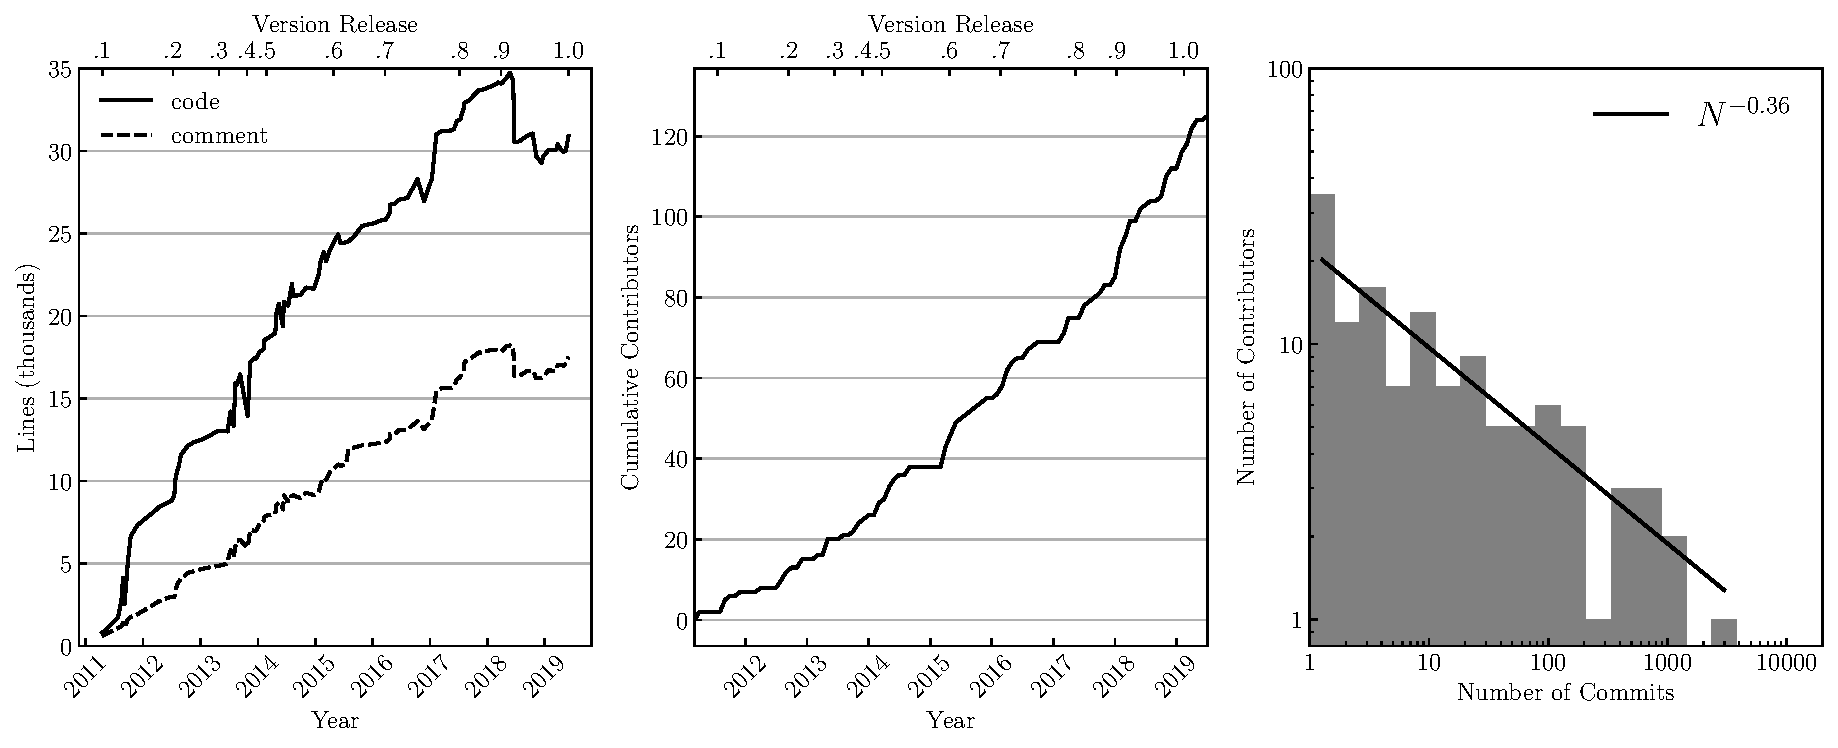
\includegraphics[width = 1.0\textwidth]{figures/dev_meta.pdf}
    \caption{Left panel: A plot of the steady increase in the total number of lines of code (solid line) and lines of comments/documentation (dotted line) as a function of time.
	Major version releases are indicated along the top axis.
	A striking reduction in the code base occurred after version 0.9.
	This period saw a major code reorganization and deletion of obsolete features along with removing support for Python~2.
	Middle panel: The cumulative number of contributors to \sunpypkg as a function of time shows a steady increase in the number of people involved in the development team.
	Right panel: A plot of the distribution of the number of commits per contributor.
	This distribution indicates that the majority of commits are undertaken by a small group of contributors. The average number of commits per contributor is less than 10 commits.}
\label{fig:metafig}
\end{figure}
